%!TEX TS-program = xelatex
%!TEX encoding = UTF-8 Unicode
% Awesome CV LaTeX Template for CV/Resume
%
% This template has been downloaded from:
% https://github.com/posquit0/Awesome-CV
%
% Author:
% Claud D. Park <posquit0.bj@gmail.com>
% http://www.posquit0.com
%
%
% Adapted to be an Rmarkdown template by Mitchell O'Hara-Wild
% 23 November 2018
%
% Template license:
% CC BY-SA 4.0 (https://creativecommons.org/licenses/by-sa/4.0/)
%
%-------------------------------------------------------------------------------
% CONFIGURATIONS
%-------------------------------------------------------------------------------
% A4 paper size by default, use 'letterpaper' for US letter
\documentclass[11pt,a4paper,]{awesome-cv}

% Configure page margins with geometry
\usepackage{geometry}
\geometry{left=1.4cm, top=.8cm, right=1.4cm, bottom=1.8cm, footskip=.5cm}


% Specify the location of the included fonts
\fontdir[fonts/]

% Color for highlights
% Awesome Colors: awesome-emerald, awesome-skyblue, awesome-red, awesome-pink, awesome-orange
%                 awesome-nephritis, awesome-concrete, awesome-darknight

\definecolor{awesome}{HTML}{207373}

% Colors for text
% Uncomment if you would like to specify your own color
% \definecolor{darktext}{HTML}{414141}
% \definecolor{text}{HTML}{333333}
% \definecolor{graytext}{HTML}{5D5D5D}
% \definecolor{lighttext}{HTML}{999999}

% Set false if you don't want to highlight section with awesome color
\setbool{acvSectionColorHighlight}{true}

% If you would like to change the social information separator from a pipe (|) to something else
\renewcommand{\acvHeaderSocialSep}{\quad\textbar\quad}

\def\endfirstpage{\newpage}

%-------------------------------------------------------------------------------
%	PERSONAL INFORMATION
%	Comment any of the lines below if they are not required
%-------------------------------------------------------------------------------
% Available options: circle|rectangle,edge/noedge,left/right

\photo{../images/JDL.jpg}
\name{Juan David}{Leongómez}

\position{Associate Professor}
\address{Faculty of Psychology, Universidad El Bosque}

\mobile{(+57) 601-6489000 Ext. 1901}
\email{\href{mailto:jleongomez@unbosque.edu.co}{\nolinkurl{jleongomez@unbosque.edu.co}}}
\homepage{jdleongomez.info}
\orcid{0000-0002-0092-6298}

% \gitlab{gitlab-id}
% \stackoverflow{SO-id}{SO-name}
% \skype{skype-id}
% \reddit{reddit-id}

\quote{I am a researcher mainly interested in human behaviour, as well
as quantitative methods and reproducible science.}

\usepackage{booktabs}

\providecommand{\tightlist}{%
	\setlength{\itemsep}{0pt}\setlength{\parskip}{0pt}}

%------------------------------------------------------------------------------



% Pandoc CSL macros
\newlength{\cslhangindent}
\setlength{\cslhangindent}{1.5em}
\newlength{\csllabelwidth}
\setlength{\csllabelwidth}{2em}
\newenvironment{CSLReferences}[3] % #1 hanging-ident, #2 entry spacing
 {% don't indent paragraphs
  \setlength{\parindent}{0pt}
  % turn on hanging indent if param 1 is 1
  \ifodd #1 \everypar{\setlength{\hangindent}{\cslhangindent}}\ignorespaces\fi
  % set entry spacing
  \ifnum #2 > 0
  \setlength{\parskip}{#2\baselineskip}
  \fi
 }%
 {}
\usepackage{calc}
\newcommand{\CSLBlock}[1]{#1\hfill\break}
\newcommand{\CSLLeftMargin}[1]{\parbox[t]{\csllabelwidth}{\honortitlestyle{#1}}}
\newcommand{\CSLRightInline}[1]{\parbox[t]{\linewidth - \csllabelwidth}{\honordatestyle{#1}}}
\newcommand{\CSLIndent}[1]{\hspace{\cslhangindent}#1}

\begin{document}

% Print the header with above personal informations
% Give optional argument to change alignment(C: center, L: left, R: right)
\makecvheader

% Print the footer with 3 arguments(<left>, <center>, <right>)
% Leave any of these blank if they are not needed
% 2019-02-14 Chris Umphlett - add flexibility to the document name in footer, rather than have it be static Curriculum Vitae
\makecvfooter
  {06 December, 2022}
    {Juan David Leongómez~~~·~~~Short Curriculum Vitae}
  {\thepage}


%-------------------------------------------------------------------------------
%	CV/RESUME CONTENT
%	Each section is imported separately, open each file in turn to modify content
%------------------------------------------------------------------------------



\hypertarget{about-me}{%
\section{About me}\label{about-me}}

\begin{minipage}[c]{0.85\linewidth}
I am an Associate Professor and Researcher at \href{https://jdleongomez.info/en/team/}{\textit{\textbf{EvoCo}: Human Behaviour and Evolution Lab}}, and leader of the \href{https://investigaciones.unbosque.edu.co/codec}{\textit{\textbf{CODEC}: Cognitive and Behavioural Sciences}} research group (classification \href{https://scienti.minciencias.gov.co/gruplac/jsp/visualiza/visualizagr.jsp?nro=00000000001446}{\textbf{A1}}), \href{https://www.uelbosque.edu.co/psicologia}{Faculty of Psychology}, at \href{https://www.uelbosque.edu.co/}{Universidad El Bosque} in Bogota, Colombia. My research interests include mate choice and human vocal communication, with an aspiration towards understanding musicality. I am also interested in bioacoustics and psychoacoustics, as well as hormonal effects on human behaviour. I published among the first articles showing within-individual changes in voice pitch in response to the social status of the listener, and have demonstrated strong effects of voice modulation on listeners in courtship contexts. I am very passionate about quantitative methods and \textbf{R} programming, as a tool to promote reproducibility and open science.
\end{minipage} \begin{minipage}[c]{0.15\linewidth}
\begin{flushright} 
\hfill \href{https://jdleongomez.info/es/team/}{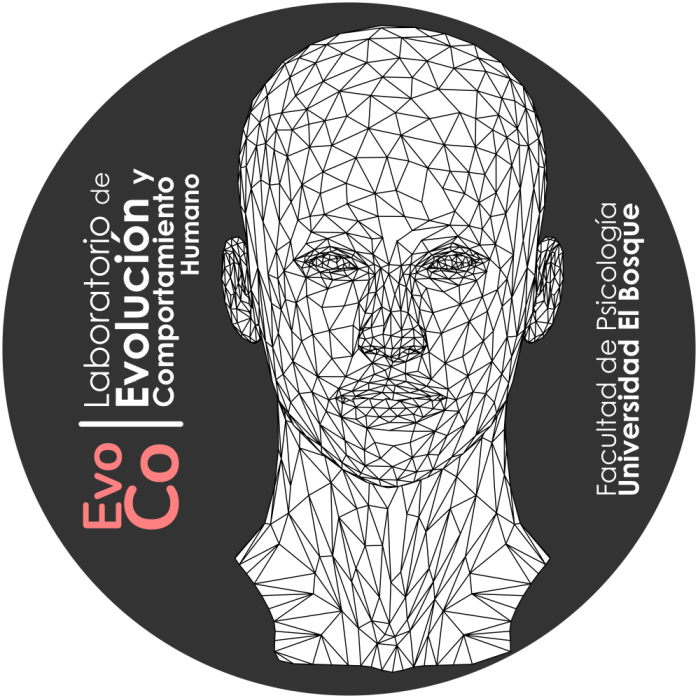
\includegraphics[width=2.3cm, height=2.3cm]{Logo_EvoCo.png}} \newline \href{https://investigaciones.unbosque.edu.co/codec}{
\includegraphics[width=2.3cm, height=2.3cm]{Logo_CODEC.png}}
\end{flushright}
\end{minipage}

\hypertarget{skills}{%
\section{Skills}\label{skills}}

\begin{cvskills}
  \cvskill
    {Programming}
    {\href{https://www.r-project.org/}{\textbf{R}} (advanced: all data wrangling, analysis, plots and tables -and even this CV- made in R)}

  \cvskill
    {Reproducible Reports}
    {Markdown/\href{https://rmarkdown.rstudio.com/}{R Markdown} (including {\fontfamily{cmr}\selectfont\LaTeX} and HTML\faHtml5). Version control with \href{https://git-scm.com/}{Git} in \href{https://github.com/JDLeongomez}{GitHub} \faGithub}

  \cvskill
    {Quantitative Research}
    {General and generalised models, linear mixed-effects models, multi-model inference, machine learning}

  \cvskill
    {Software}
    {\href{https://posit.co/products/open-source/rstudio/}{RStudio}, \href{https://code.visualstudio.com/}{Visual Studio Code}, \href{https://www.fon.hum.uva.nl/praat/}{Praat}, \href{https://www.audacityteam.org/}{Audacity}, \href{https://inkscape.org/}{InkScape}, \href{https://www.zotero.org/}{Zotero}}

  \cvskill
    {Languages}
    {English/Spanish (native)}
\end{cvskills}

\hypertarget{education}{%
\section{Education}\label{education}}

\begin{cventries}
    \cventry{PhD - Psychology}{\href{https://www.stir.ac.uk/}{University of Stirling}}{Stirling, UK}{2014}{}\vspace{-4.0mm}
    \cventry{MSc in Evolutionary Psychology}{\href{https://www.liverpool.ac.uk/}{University of Liverpool}}{Liverpool, UK}{2009}{}\vspace{-4.0mm}
    \cventry{BA in Music Pedagogy}{\href{https://www.upn.edu.co/}{Universidad Pedagógica Nacional}}{Bogota, Colombia}{2006}{}\vspace{-4.0mm}
\end{cventries}

\hypertarget{working-and-teaching-experience}{%
\section{Working and Teaching
Experience}\label{working-and-teaching-experience}}

For a full list, and a description of responsibilities, please check
\href{https://jdleongomez.info/en/profile/\#experience}{my website} or
my \href{https://jdleongomez.info/en/files/jdl_cv_en.pdf}{academic CV}.

\begin{cventries}
    \cventry{Associate Professor}{\href{https://www.unbosque.edu.co/}{Universidad El Bosque}}{Bogota, Colombia}{Jan. 2015 - Present}{}\vspace{-4.0mm}
\end{cventries}

\hypertarget{accomplishments}{%
\section{Accomplishments}\label{accomplishments}}

For information on \textbf{grants}, \textbf{scholarships},
\textbf{awards} and \textbf{prizes}, please check
\href{https://jdleongomez.info/en/profile/\#accomplishments}{my website}
or my \href{https://jdleongomez.info/en/files/jdl_cv_en.pdf}{academic
CV}.

\hypertarget{selected-publications}{%
\section{Selected Publications}\label{selected-publications}}

For a full list, please check the publications section on
\href{https://jdleongomez.info/en/publication/}{my website} or my
\href{https://jdleongomez.info/en/files/jdl_cv_en.pdf}{academic CV}.

\begingroup
\setlength{\parindent}{-0.5in}
\setlength{\leftskip}{0.5in}

\textbf{Leongómez, J. D.}, Havlíček, J., \& Roberts, S. C. (2022).
Musicality in Human Vocal Communication: An Evolutionary Perspective.
\emph{Philosophical Transactions of the Royal Society B: Biological
Sciences, 377}, 20200391. \url{https://doi.org/10.1098/rstb.2020.0391}

Kleisner, K., \textbf{Leongómez, J. D.}, Pisanski, K., Fiala, V.,
Cornec, C., Groyecka, A., \ldots{} Akoko, R. M. (2021). Predicting
strength from aggressive vocalisations versus speech in African bushland
and urban communities. \emph{Philosophical Transactions of the Royal
Society B: Biological Sciences, 376}, 20200403.
\url{https://doi.org/10.1098/rstb.2020.0403}

\textbf{Leongómez, J. D.}, Pisanski, K., Reby, D., Sauter, D., Lavan,
N., Perlman, M., \& Varella Valentova, J. (2021). Voice modulation: From
origin and mechanism to social impact. \emph{Philosophical Transactions
of the Royal Society B: Biological Sciences, 376}, 20200386.
\url{https://doi.org/10.1098/rstb.2020.0386}

\textbf{Leongómez, J. D.}, Sánchez, O. R., Vásquez-Amézquita, M., \&
Roberts, S. C. (2021). Contextualising courtship: Exploring male body
odour effects on vocal modulation. \emph{Behavioural Processes, 193},
104531. \url{https://doi.org/10.1016/j.beproc.2021.104531}

\textbf{Leongómez, J. D.}, Sánchez, O. R., Vásquez-Amézquita, M.,
Valderrama, E., Castellanos-Chacón, A., Morales-Sánchez, L., \ldots{}
González-Santoyo, I. (2020). Self-reported Health is Related to Body
Height and Waist Circumference in Rural Indigenous and Urbanised
Latin-American Populations. \emph{Scientific Reports, 10}, 4391.
\url{https://doi.org/10.1038/s41598-020-61289-4}

\textbf{Leongómez, J. D.}, Mileva, V. R., Little, A. C., \& Roberts, S.
C. (2017). Perceived differences in social status between speaker and
listener affect the speaker's vocal characteristics. \emph{PLOS One,
12}(6), e0179407. \url{https://doi.org/10.1371/journal.pone.0179407}

\textbf{Leongómez, J. D.}, Binter, J., Kubicová, L., Stolařová, P.,
Klapilová, K., Havlíček, J., \& Roberts, S. C. (2014). Vocal modulation
during courtship increases proceptivity even in naive listeners.
\emph{Evolution and Human Behavior, 35}(6), 489--496.
\url{https://doi.org/10.1016/j.evolhumbehav.2014.06.008}

\endgroup

\begin{footnotesize}
\textbf{Note:} I am the/a corresponding author in all these publications
\end{footnotesize}

\hypertarget{investigaciuxf3n-abierta-youtube-channel}{%
\section{Investigación Abierta (YouTube
channel)}\label{investigaciuxf3n-abierta-youtube-channel}}

\begin{minipage}[c]{0.15\linewidth}
\href{https://www.youtube.com/@InvestigacionAbierta}{
\includegraphics[width=2cm, height=2cm]{Logo_IA.png}}
\end{minipage} \begin{minipage}[c]{0.85\linewidth}
\textcolor{red}{\faYoutubePlay} \href{https://www.youtube.com/@InvestigacionAbierta}{Investigación Abierta} [\textit{Open Research}] is a YouTube channel (in Spanish) where I post videos and tutorials related to quantitative research methods and open science, as well as useful open source software.
\end{minipage}

\hypertarget{postgraduate-supervision}{%
\section{Postgraduate Supervision}\label{postgraduate-supervision}}

For a full list, including undergraduate supervision, please check
\href{https://jdleongomez.info/en/team/}{my website} or my
\href{https://jdleongomez.info/en/files/jdl_cv_en.pdf}{academic CV}.

\begin{cventries}
    \cventry{PhD in Neuroscience}{\href{https://www.researchgate.net/profile/Milena-Vasquez-Amezquita}{Milena Vásquez-Amézquita}}{\href{https://www.uv.es/}{Universitat de València}, Spain}{2015 - 2018}{\begin{cvitems}
\item Supervised together with  Alicia Salvador
\end{cvitems}}
    \cventry{Professional Doctorate in Counselling Psychology}{\href{https://www.researchgate.net/profile/Francisco-Flores-14}{Francisco Javier Flores}}{\href{https://www.uel.ac.uk/}{University of East London}, UK}{2015 - 2018}{\begin{cvitems}
\item Supervised together with Lisa Chiara Fellin
\end{cvitems}}
    \cventry{Psychological Research Methods (Evolutionary Psychology) MSc}{Julia Sanz-Vidania}{\href{https://www.stir.ac.uk/}{University of Stirling}, UK}{2013 - 2014}{\begin{cvitems}
\item Supervised together with \href{https://www.scraigroberts.com/}{S Craig Roberts}
\end{cvitems}}
\end{cventries}

\hypertarget{editorial-appointments}{%
\section{Editorial Appointments}\label{editorial-appointments}}

I recently served as a guest editor of a 2-part theme issue on
\href{https://royalsocietypublishing.org/journal/rstb}{Philosophical
Transactions B} (check
\href{https://royalsocietypublishing.org/toc/rstb/2021/376/1840}{Part
1},
\href{https://royalsocietypublishing.org/toc/rstb/2022/377/1841}{Part
2}). I have served as an \textit{ad-hoc} reviewer for a variety of
journals including
\href{https://royalsocietypublishing.org/journal/rspb}{Proceedings of
the Royal Society B: Biological Sciences},
\href{https://royalsocietypublishing.org/journal/rsos}{Royal Society
Open Science}, \href{https://journals.plos.org/plosone/}{PLOS ONE},
\href{https://www.sciencedirect.com/journal/evolution-and-human-behavior}{Evolution
and Human Behavior}, \href{https://www.nature.com/srep/}{Scientific
Reports}, \href{https://www.tandfonline.com/toc/hbas20/current}{Basic
and Applied Social Psychology},
\href{https://www.journals.elsevier.com/cortex}{Cortex\}},
\href{https://journals.sagepub.com/home/pec}{Perception},
\href{https://journals.sagepub.com/home/evp}{Evolutionary Psychology},
and \href{https://www.frontiersin.org/journals/psychology}{Frontiers in
Psychology} where I am currently a
\href{https://loop.frontiersin.org/people/438954/overview}{Review
Editor} for the
\href{https://www.frontiersin.org/journals/psychology/sections/evolutionary-psychology}{\textit{Evolutionary Psychology specialty section}}.
My full, verified review record is available from my
\href{https://www.webofscience.com/wos/author/record/387716}{Web of
Science} profile.



\end{document}
